\chapter{O algoritmo de Viola e Jones}\label{cap:viola_jones}

O algoritmo apresentado por Paul Viola e Michael J. Jones em 2001 \cite{Viola01rapidobject} \cite{viola2004robust} e revisado em 2003 \cite{jones2003fast} obteve grande sucesso pela sua relativa simplicidade, rápida execução e notável performance \cite{jensen2008implementing}. Ele encontra-se implementado na biblioteca OpenCV \cite{bradski2000intel} \cite{opencvdocs} e, além de detectar faces, também pode ser treinado para detecção objetos diversos.

O processo de treino é lento, porém a detecção é bastante rápida. De acordo com \citeonline{omaia2009sistema}, "este foi o primeiro método de detecção de face em tempo real em vídeo, conseguindo processar até 15 quadros por segundo".

De acordo com \cite{zhang2010survey} e \cite{Viola01rapidobject}, o algoritmo, na forma como proposto no artigo original, possui baixas taxas de detecção para faces de perfil ou inclinadas. Essa limitação foi tratada pelos autores na revisão de 2003 \cite{jones2003fast} e também por outros pesquisadores, porém essas variantes fogem do escopo deste trabalho.

O detector de faces de Viola-Jones possui quatro estágios: seleção de características Haar-like retangulares, criação da imagem integral, que permite o cálculo rápido das características, treino de classificadores por um algoritmo de aprendizado de máquina baseado no AdaBoost e, por fim, o uso de classificadores em cascata, que descarta as regiões de fundo para focar em áreas mais prováveis de conter uma face.


\section{Características Haar-like retangulares}\label{sec:haar_features}

As características de Haar utilizadas por Viola-Jones, ilustradas na Figura \ref{fig:haar_like_features}, foram inspiradas nos trabalhos de \citeonline{papageorgiou1998general}, que descreveram características construídas a partir de um conjunto de ondaletas de Haar (Haar wavelets).

\begin{figure}[htbp]
   \begin{center}
     
\includegraphics{imagens/haar_like_features.png}
   \end{center}
   \caption{Características Haar-like \label{fig:haar_like_features}}
\end{figure}

As características Haar-like consistem em um ou mais retângulos adjacentes e são utilizadas para analisar locais específicos em uma janela de detecção. Cada característica resulta em um único valor, calculado através da soma das intensidades dos pixels sob os retângulos brancos subtraída da soma dos valores sob os retângulos pretos, como na Equação \ref{eq:calc_haar_feature}:
%
\begin{equation} \label{eq:calc_haar_feature}
\Delta = \frac{1}{n}  \sum_{preto}^{n} I(x) - \frac{1}{n}  \sum_{branco}^{n} I(x)
\end{equation}
%
Quanto mais próximo de 1, mais semelhante é a imagem real da característica aplicada.

\begin{figure}[htbp]
    \begin{subfigure}[c]{0.45\textwidth}
    \centering
    \begin{tikzpicture}
    \matrix[square matrix, text=cyan] {
        0 & 0 &|[fill=black]| 1 &|[fill=black]| 1 \\
        0 & 0 &|[fill=black]| 1 &|[fill=black]| 1 \\
        0 & 0 &|[fill=black]| 1 &|[fill=black]| 1 \\
        0 & 0 &|[fill=black]| 1 &|[fill=black]| 1 \\
    };
    \end{tikzpicture}
    \caption{Intensidades ideais}
    \end{subfigure}
    \begin{subfigure}[c]{0.45\textwidth}
    \centering
    \begin{tikzpicture}
    \matrix[square matrix, text=cyan] {
        |[fill=black!20]|0.2 &|[fill=black!20]| 0.2 &|[fill=black!80]| 0.8 &|[fill=black!60]| 0.6 \\
        |[fill=black!10]|0.1 &|[fill=black!30]| 0.3 &|[fill=black!60]| 0.6 &|[fill=black!80]| 0.8 \\
        |[fill=black!20]|0.2 &|[fill=black!10]| 0.1 &|[fill=black!80]| 0.8 &|[fill=black!80]| 0.8 \\
        |[fill=black!20]|0.2 &|[fill=black!10]| 0.1 &|[fill=black!60]| 0.6 &|[fill=black!90]| 0.9 \\
    };
    \end{tikzpicture}
    \caption{Valores reais}
    \end{subfigure}
    \caption{Exemplo de característica aplicada a uma imagem real. Pela Equação \ref{eq:calc_haar_feature}, $\Delta = 0,74 - 0,18 = 0,56$.}
\end{figure}

Utilizar características é mais vantajoso do que trabalhar com cada pixel da imagem separadamente, pois é menos custoso computacionalmente e elas permitem reconhecer padrões determinados. A característica 2 da Figura \ref{fig:haar_like_features} pode ser utilizada para reconhecer a região dos olhos, que costuma ser mais escura do que a região das bochechas, e a característica 3 pode ser usada para reconhecer a região do nariz, como mostrado na figura \ref{fig:julio_haar}.

Existem alternativas mais sofisticadas às características Haar-like, como filtros orientáveis (steerable filters) \cite{freeman1991design} \cite{greenspan1994overcomplete}, porém, segundo \citeonline{Viola01rapidobject}, a eficiência de características retangulares fornece ampla compensação por sua flexibilidade limitada.

\begin{figure}[htbp]
   \begin{center}
     \scalebox{0.25}{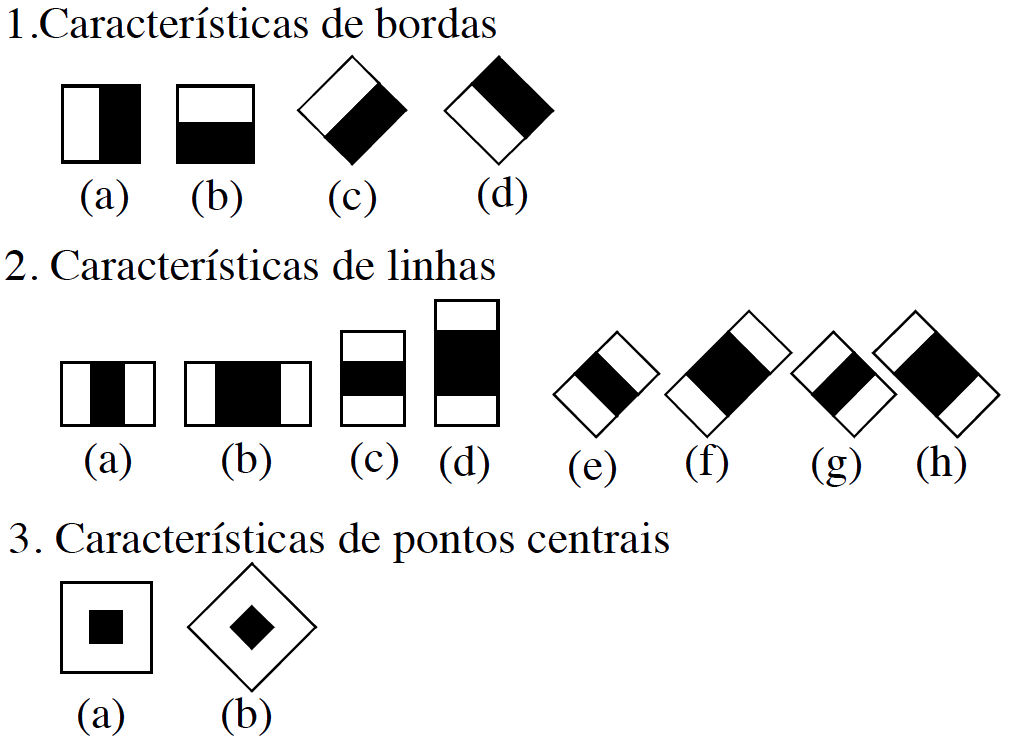
\includegraphics{imagens/lienhart_haar_features.png}}
   \end{center}
   \caption{Características propostas por Lienhart e Maydt \label{lienhart_haar_features}}
\end{figure}

Em \citeonline{lienhart2002extended} foram propostas novas características contendo rotações de \ang{45}, mostradas na Figura \ref{lienhart_haar_features}. Segundo os autores, o uso dessas características reduziu em 10\%, em média, o número de alarmes falsos. \citeonline{messom2009stream} estenderam essa ideia para rotações de qualquer ângulo, ao custo dos erros de arredondamento.

\begin{figure}[htbp]
    \begin{subfigure}[c]{0.3\textwidth}
    \centering
    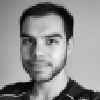
\includegraphics{imagens/julio_haar1.png}
    \caption{}
    \end{subfigure}
    \begin{subfigure}[c]{0.3\textwidth}
    \centering
    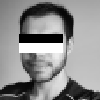
\includegraphics{imagens/julio_haar2.png}
    \caption{}
    \end{subfigure}
    \begin{subfigure}[c]{0.3\textwidth}
    \centering
    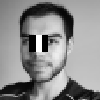
\includegraphics{imagens/julio_haar3.png}
    \caption{}
    \end{subfigure}
    \caption{Características usadas para detectar olhos e nariz}
    \label{fig:julio_haar}
\end{figure}

Para uma imagem com resolução de $24\times24$ px, pode-se construir dezenas de milhares de características diferentes considerando todas as variações de tamanho e posição das características na Figura \ref{fig:haar_like_features}. Para calcular todas elas de forma eficiente, é usada uma representação intermediária da imagem, chamada imagem integral.


\section{Imagem Integral}\label{sec:imagem_integral}

O algoritmo da imagem integral, proposto por \citeonline{crow1984summed} para mapeamento de texturas (mipmaps), é capaz de calcular rapidamente a soma dos valores em um subconjunto retangular de uma matriz.

A imagem integral é uma tabela bidimensional do tamanho da imagem original, onde cada elemento equivale à soma de todos os níveis de cinza (intensidades) dos pixels à esquerda e acima do pixel atual, inclusive. Ela pode ser descrita pela equação \ref{eq:imagemintegral}:
%
\begin{equation} \label{eq:imagemintegral}
    ii(x,y) = \sum_{{x}'\leq x, {y}'\leq y} i({x}', {y}')
\end{equation}
%
onde $ii(x,y)$ é a imagem integral e $i(x,y)$ é a imagem original.

\begin{figure}[htbp]
    \begin{subfigure}[c]{0.3\textwidth}
    \centering
    \begin{tikzpicture}
    \matrix[square matrix=1.7em] (m){
        0.1 & 0.1 & 0.2 & 0.1 & 0.7 \\
        0.2 & 0.3 & 0.2 & 0.7 & 0.8 \\
        0.1 & 0.4 & 0.3 & 0.3 & 0.1 \\
        0.1 & 0.5 & 0.1 & 0.1 & 0.2 \\
        0.1 & 0.4 & 0.8 & 0.5 & 0.6 \\
    };
    \end{tikzpicture}%
    \caption{Imagem original}
    \end{subfigure}%
    \begin{subfigure}[c]{0.3\textwidth}
    \centering
    \begin{tikzpicture}
    \matrix[square matrix=1.7em, opacity=0.8] (m){
        0.1 & 0.1 & 0.2 & 0.1 & 0.7 \\
        0.2 & 0.3 & 0.2 & 0.7 & 0.8 \\
        0.1 & 0.4 & 0.3 & 0.3 & 0.1 \\
        0.1 & 0.5 & 0.1 & 0.1 & 0.2 \\
        0.1 & 0.4 & 0.8 & 0.5 & 0.6 \\
    };
    \filldraw[fill=yellow, fill opacity=0.2, text opacity=1] (m-2-3.north west) rectangle (m-4-4.south east);% node[pos=.5] {D};
    \fill[blue] (m-1-2.south east) circle(2pt) node[left, font=\small] {\textbf{A}};
    \fill[blue] (m-1-4.south east) circle(2pt) node[right, font=\small] {\textbf{B}};
    \fill[blue] (m-4-2.south east) circle(2pt) node[left, font=\small] {\textbf{C}};
    \fill[blue] (m-4-4.south east) circle(2pt) node[right, font=\small] {\textbf{D}};
    \end{tikzpicture}%
    \caption{Região de interesse}
    \end{subfigure}%
    \begin{subfigure}[c]{0.3\textwidth}
    \centering
    \begin{tikzpicture}
    \matrix[square matrix=1.7em] (m){
        0.1 & 0.2 & 0.4 & 0.5 & 1.2 \\
        0.3 & 0.7 & 1.1 & 1.9 & 3.4 \\
        0.4 & 1.2 & 1.9 & 3.0 & 4.6 \\
        0.5 & 1.7 & 2.5 & 3.7 & 5.3 \\
        0.6 & 2.3 & 3.9 & 5.6 & 8.0 \\
    };
    \filldraw[fill=yellow, fill opacity=0.2] (m-1-2.north west) rectangle (m-1-2.south east);
    \filldraw[fill=yellow, fill opacity=0.2] (m-1-4.north west) rectangle (m-1-4.south east);
    \filldraw[fill=yellow, fill opacity=0.2] (m-4-2.north west) rectangle (m-4-2.south east);
    \filldraw[fill=yellow, fill opacity=0.2] (m-4-4.north west) rectangle (m-4-4.south east);
    \draw[blue,<-,shorten <=1pt] (m-1-2)
    |- +(0.2,0.8)
    node[right] {$ii(A)$};
     \draw[blue,<-,shorten <=1pt] (m-1-4)
    |- +(0.2,0.8)
    node[right] {$ii(B)$};
    \draw[blue,<-,shorten <=1pt] (m-4-2)
    |- +(0.2,-1.4)
    node[right] {$ii(C)$};
    \draw[blue,<-,shorten <=1pt] (m-4-4)
    |- +(0.2,-1.4)
    node[right] {$ii(D)$};
    \end{tikzpicture}%
    \caption{Imagem integral}
    \end{subfigure}%
    \caption{Imagem ilustrada como matriz de pixels}
    \label{fig:imagem_integral}
\end{figure}

Utilizando a imagem integral, a soma dos níveis de cinza de qualquer área retangular pode ser calculada em quatro referências à memória. A soma dos valores na região ABCD da Figura \ref{fig:imagem_integral} pode ser rapidamente calculada como mostrado na equação \ref{eq:ii_calculo_regiao_abcd}:
%
\begin{align} \label{eq:ii_calculo_regiao_abcd}
    \sum_{(x,y) \in ABCD} i(x,y) &= ii(D) + ii(A) - (ii(B) + ii(C))\\
                                 &= 3,7 + 0,2 - (0,5 + 1,7) = 1,7\nonumber
\end{align}

O cálculo de características compostas por dois retângulos (1 e 2 da \ref{fig:haar_like_features}), requerem seis referências à memória, as características compostas por três retângulos (3) requerem oito acessos e as compostas por quatro retângulos (4) requer nove acessos.


\section{AdaBoost}\label{sec:adaboost}

Apesar do cálculo de cada característica ser rápido, calcular todo o conjunto de características é inviável. Experimentalmente descobriu-se que um classificador eficiente pode ser formado combinando um pequeno subconjunto com apenas as características mais representativas. O algoritmo de Viola-Jones utiliza uma variante do AdaBoost para selecionar essas características e treinar o classificador.

O AdaBoost é um método de aprendizado de máquina, inventado por Yoav Freund e Robert Schapire\cite{freund1997decision}, que combina de forma ponderada vários classificadores fracos com taxa de acerto acima de 50\% para obter um classificador forte.

Um classificador fraco $h_{j}(x)$ consiste em uma característica $f_{j}$, um limite $\theta_{j}$ e uma paridade $p_{j}$, que indica a direção da desigualdade:
%
\begin{equation} \label{eq:weak_classifier}
    h_{j}(x) = 
    \begin{cases}
        1 & \text{se } p_{j}f_{j}(x) < p_{j}\theta_{j}\\
        0 & \text{caso contrário}
    \end{cases}
\end{equation}
%
onde $x$ é uma janela de $24\times24$ px de uma imagem.

